\setcounter{chapter}{-1}

\chapter{Getting started}
\label{cha:getting-started}

\minitoc

\begin{note}
  This is where the script for the first, one hour lab, should go. The text below is the pre-reading document we handed out last year in first lab session

  Need to think how we deliver this material to students. Paper? Web?  If latter, then how do they find out where?

  It should cover the following
  \begin{enumerate}
  \item Rebooting into Windows
  \item Logging in to Windows
  \item Reading mail through My Manchester
  \item Getting IMAP settings
  \item Mail IMAP settings to self
  \item Set up mail reading on phone, if have one
  \item Rebooting into Linux
  \item Read Intro material on Unix
  \end{enumerate}
\end{note}


\section{Using Windows}
\label{sec:using-windows}
  \begin{enumerate}
  \item Rebooting into Windows
  \item Logging in to Windows
  \end{enumerate}


\subsection{Reading your mail}
\label{sec:reading-your-mail}
  \begin{enumerate}
  \item Reading mail through My Manchester
  \item Getting IMAP settings
  \item Mail IMAP settings to self
  \item Set up mail reading on phone, if have one
  \end{enumerate}

\subsection{Rebooting into Linux}
\label{sec:rebooting-into-linux}
  \begin{enumerate}
  \item Rebooting into Linux
  \item Read Intro material on Unix
  \end{enumerate}


\section{Using the School Linux system}

Over the next couple of weeks you will be undertaking a number of introductory labs to familiarise yourself with the School's computing infrastructure. Much of this is based on machines running Linux, a variant of the Unix family of operating systems; this document provides some background on Unix and explains why we think it is important. It would very useful if you could read this before you attend the first introductory labs, where the emphasis will be on leading you through a series of tasks to explore our setup.

\section{Operating Systems}

An \wikipedia{Operating_system}{operating system} (OS) is a suite of software that makes
computer hardware usable; it makes the `raw computing power' of the
hardware available to the user. You're probably most familiar with the \wikipedia{Microsoft_windows}{Microsoft Windows} and Apple \wikipedia{OS_X}{OS X} families of operating systems for `desktop' computers, and \wikipedia{Ios}{iOS} (Apple, again) and Google's \wikipedia{Android_(operating_system)}{Android} for mobile devices; but many other more specialist operating systems exist, and you'll be studying some of these and the principles that underpin OS design in COMP25111 in your second year. In the meantime, a potted history of OS development will tide us over\ldots
 
\section{Unix Origins}
\label{sec:unix}


In the late 1950s, an American company called \wikipedia{Bell_Labs}{Bell Laboratories} decided that they needed a system to improve the way they worked with their computer hardware (it's probably quite hard to imagine what interacting with a computer \emph{without} an operating system might be; but it wasn't pretty and involved manually loading and running programs one by one). Together with the \wikipedia{General_Electric_Company}{General Electric Company} and the \wikipedia{MIT}{Massachusetts Institute of Technology}, they set about the design of an operating system they called \wikipedia{Multics}{Multics}: the `Multiplexed Information and Computing Service'. Multics was hugely innovative, and introduced many concepts that we now take for granted in modern operating systems such as the ability for more than one program to run `at once'; but it did rather suffer from `design by committee', and the final system was seen at the time as being overly complex and rather bloated (`bloated' is all a matter of perspective of course: its sobering to realise though that the entire Multics operating system was only around 135Kb. Today's operating systems are something like 30,000 times this size\ldots). In the late 1960s, a group of programmers at Bell Labs created a cut-down, leaner and cleaner version of Multics that would work on more modest hardware. Legend has it that this was to allow them to play their favourite (only!) computer game, \wikipedia{Space_Travel_(video_game)}{Space Travel}. In an early example of the trend of giving things `punny' names, to contrast with the more clumsy Multics, they called this new system Unix. The so-called \wikipedia{Jargon_File}{Jargon File} is a good source of explanations of various bits of computer slang and their obscure origins, and is well worth a read: in part to give some background history, but mostly as an insight into the minds of the computing pioneers of the past!

%\begin{htmlonly}
%(See the Unix entry in the useful and amusing
%\htmladdnormallink{Jargon
%file}{http://www.new.ox.ac.uk/admin/jargon/html/entry/Unix.html}, a
%file}{http://www.cs.manchester.ac.uk/software/jargon/html/entry/Unix.html}, a
%file}{\jargonFileUnix}, a
%`collection of slang terms used by various subcultures of computer
%\htmladdnormallink{hackers}
%{http://www.cs.manchester.ac.uk/software/jargon/html/entry/hacker.html}'.)
%{\jargonFileHackers}'.)
%\end{htmlonly}

Even though Unix is now quite old, most Computer Scientists recognise that the designers of Unix got most of the fundamental concepts and
architecture right. Given how much computing has changed since the 1960s, this was an astonishing intellectual achievement. Although Microsoft's \wikipedia{Microsoft_Windows}{Windows} is by far the most common operating system on \emph{desktop} machines, the majority of the Internet, much of the world's corporate infrastructure, virtually all supercomputers, and even some mobile devices are powered by Unix-like operating systems. So, while the polished graphical user interfaces of Windows and \wikipedia{OS_X}{OS X} appear to dominate the world of computing, most of the real hard-core and leading-edge computation relies on an elegant operating system designed nearly 50 years ago (by a team of scientists who wanted to play a game).  

\section{Modern Unix Variants}
\label{sec:modern-unix-variants}


The history of Unix is complex and convoluted, with the system being updated, re-implemented, and mimicked repeatedly over the years, primarily by commercial companies who guarded their versions jealously. Figure \ref{fig:unix-history} shows a tiny fragment of the Unix's `family tree' (the full diagram, which you can find at \urlnop{www.levenez.com/unix/unix.pdf}, is \emph{many} times the size of the portion you can see here).

\begin{figure}[h!tb]
  \begin{center}
    \includegraphics[width=13cm]{images/unix}
  \end{center}
\caption{A fragment of \'{E}ric L\'{e}v\'{e}nez's Unix History chart, reproduced with permission and showing the beginnings of Linux in amongst other versions of Unix.}
\label{fig:unix-history}
\end{figure}
 
Although many of the branches represent interesting innovations of one kind or another, there are perhaps two that deserve particular attention. The first of these was the decision by Apple some time around the turn of the millenium to drop their own---highly popular, but aging---bespoke operating system (unimaginatively called \wikipedia{Mac_os_9}{Mac OS 9}) in favour of a Unix-based system (now the more familiar `OS X', where `X' is both the Roman numeral `10' and a nod in the direction of the uniX nature of the OS). Although the majority of Mac users are blissfully unware of the fact, behind the slick front-end of OS X, sits a variant of Unix. The second, and perhaps more profound of these events was the creation in 1991 by Swedish programmer \wikipedia{Linus_torvalds}{Linus Torvalds} of a Unix-like system, the source code to which \emph{he gave away for free}\footnote{`free' here in the sense both of `freedom to reuse or adapt', and also in the sense of `without charge'.}; this became known as the \wikipedia{Linux_kernel}{Linux Kernel}. Combined with other free software created by the \wikipedia{Free_software_foundation}{Free Software Foundation}, a non-commercial version of Unix called \wikipedia{GNU/Linux}{GNU/Linux} was born (GNU here is a recursive acronym for ``GNU's not Unix'', a swipe at other commercial non-Free versions; much to the annoyance of the Free Software Foundation, GNU/Linux is almost always called just `Linux'\footnote{Linux
is pronounced ``Linn-ucks'', despite the fact the name was coined by
its creator, and his name `Linus' is pronounced
``Leen-uss''!}.) 

Linux has been, and continues to be, developed cooperatively by
thousands of programmers across the world contributing their effort
largely free of charge. It is amazing to think that such
a project could ever happen---and it is surely a testament to the
better side of Human nature. But what is interesting is the
observation that these programmers are not motivated by commercial
concerns, but by the desire to make good reliable software and have it
used by lots of people. Thus, Linux is a good choice of Unix: it's
Free, it's efficient, and it's reliable, and it is now used by large corporations, governments, research labs and individuals around the world. Even Google's \wikipedia{Android_(operating_system)}{Android} platform is a Linux-based mobile OS, and the  \wikipedia{Amazon_Kindle}{Amazon Kindle} is also a Linux box behind the electronic ink of its user interface (Figure \ref{fig:kindlelinux}).

\begin{figure}[h!tb]
  \begin{center}
    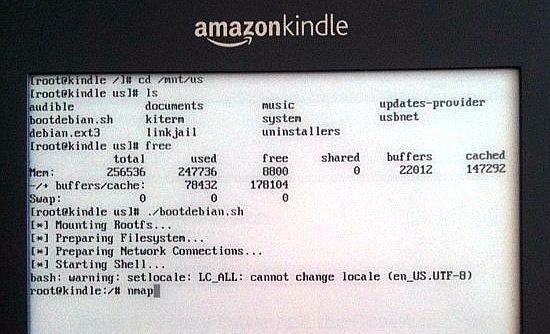
\includegraphics[width=13cm]{images/kindleroot}
  \end{center}
\caption{A photograph of Liraz Siri's `rooted' kindle, showing the Linux command prompt. Reproduced with the author's kind permission from \urlnop{www.turnkeylinux.org/blog/kindle-root}}
\label{fig:kindlelinux}
\end{figure}

One of the results of the fact that Linux is Free is that several
organisations and companies have created their own distributions of
it; these vary a bit (in fact, anybody is free to make any change they
like to Linux, and pass it on to whoever wants it). The distribution
we use in this School is \textbf{Fedora}, which is
one of the most popular and is sponsored by a
US company called \textbf{Red Hat}.
%, which is the latest release

So, if you are to become an expert computer professional, it is
important that you understand the theory and practice of Unix based
systems. Learning Unix is not only a crucial skill for any serious
computer scientist, it is a very rewarding experience; the labs over
the next couple of weeks are designed to help you become familiar with what will be your daily working environment.

